% =====================================================================
%  Trabalho do Grau B
%  Redes de Computadores: Internetworking, Roteamento e Transmissao
%  Prof. Dr. Rodolfo Stoffel Antunes (rsantunes@unisinos.br)
%
%  Caso 14: Cortes de cabos submarinos no Mar Vermelho (24/02/2024)
%  Familia C: falhas fisicas e de transmissao
% =====================================================================
\documentclass[12pt]{article}

\newif\ifsbc
\IfFileExists{sbc-template.sty}{\sbctrue}{\sbcfalse}
\ifsbc
  \usepackage{sbc-template}
  % Correcao de um defeito do sbc-template.sty (v2017). Nao remover.
  \AddToHook{begindocument/before}[sbc-template]{{}}
\else
  \usepackage[a4paper,margin=2.5cm]{geometry}
  \usepackage{times}
  \newcommand{\address}[1]{\def\sbcaddress{#1}}
  \newcommand{\inst}[1]{\textsuperscript{#1}}
  \newcommand{\email}[1]{\texttt{#1}}
  \newenvironment{resumo}{\begin{center}\bfseries Resumo\end{center}\begin{quotation}}{\end{quotation}}
  \makeatletter
  \renewcommand{\maketitle}{\begin{center}{\Large\bfseries\@title\par}\vspace{1em}{\@author\par}\vspace{.5em}{\small\sbcaddress\par}\end{center}}
  \makeatother
  \typeout{AVISO: sbc-template.sty nao encontrado, usando fallback para rascunho.}
\fi

\usepackage[utf8]{inputenc}
\usepackage[T1]{fontenc}
\usepackage[brazil]{babel}
\usepackage{graphicx}
\usepackage{booktabs}
\usepackage{tabularx}
\usepackage{url}
\urlstyle{rm}
\usepackage{xcolor}
\usepackage{tikz}
\usetikzlibrary{positioning,arrows.meta,fit,backgrounds}
\usepackage{hyperref}
\hypersetup{colorlinks=true,linkcolor=black,citecolor=black,urlcolor=blue!60!black}

% Marcadores para a linha do tempo (pergunta 1)
\newcommand{\evC}{\textbf{C}}   % confirmado pelo operador
\newcommand{\evO}{\textbf{O}}   % observado por terceiros
\newcommand{\evI}{\textbf{I}}   % inferido pelo grupo

\sloppy

% ---------------------------------------------------------------------
\title{Post-Mortem: Cortes dos cabos SEACOM/TGN-EA e AAE-1\\no Mar Vermelho, 24 de fevereiro de 2024}

\author{Ana Clara Anderle\inst{1}, Carolina Silva dos Santos\inst{1},
  Guilherme Menna Barreto da Silva\inst{1},\\ Lucas de Paula da Silva\inst{1},
  Otto Schmitz\inst{1}, Paola Spielmann Hoffmeister\inst{1}}

\address{Curso de Ci\^encia da Computa\c{c}\~ao -- Universidade do Vale do Rio dos Sinos\\
  S\~ao Leopoldo -- RS -- Brasil
  \email{\{[[login1]], [[login2]], [[login3]], [[login4]], [[login5]], [[login6]]\}@edu.unisinos.br}
}

\begin{document}
\maketitle

\begin{abstract}
  On 24 February 2024, at about 09:46 and 09:51~UTC, the SEACOM/TGN-EA and AAE-1
  submarine cables were cut in the southern Red Sea, where EIG was already down.
  Networks in East Africa, Djibouti, Saudi Arabia, the UAE and Vietnam lost transit
  from Tata, Cogent, Arelion and NTT; BGP moved multihomed networks to other upstreams
  within minutes, while single-upstream prefixes were withdrawn. User impact was short,
  but repairs took months. The likely trigger, the dragged anchor of the MV
  \textit{Rubymar}, was never confirmed. Root cause: logical upstream diversity without
  physical diversity.
\end{abstract}

\begin{resumo}
  Em 24/02/2024, por volta de 09:46 e 09:51~UTC, os cabos SEACOM/TGN-EA e AAE-1 foram
  rompidos no sul do Mar Vermelho, onde o EIG já estava fora desde dezembro de 2023.
  Redes da África Oriental, de Djibuti, da Arábia Saudita, dos Emirados e do Vietnã
  perderam trânsito da Tata, da Cogent, da Arelion e da NTT; o BGP migrou as redes com
  mais de um \textit{upstream} em minutos, e prefixos anunciados por um único provedor
  foram retirados. O impacto para usuários foi curto e localizado, mas o reparo físico
  levou meses, por depender de permissões em águas do Iêmen. O gatilho provável, a âncora
  arrastada do navio \textit{Rubymar}, abandonado após um ataque, não foi confirmado
  oficialmente. A causa raiz de engenharia é a diversidade lógica de provedores sem
  diversidade física: trânsitos ``independentes'' compartilhavam o mesmo corredor.
\end{resumo}

% =====================================================================
\section{Contexto e impacto}

O sul do Mar Vermelho, entre o Iêmen e Djibuti, é passagem obrigatória dos cabos que
ligam a Europa (via Egito) à Ásia e à costa leste da África: mais de 15 sistemas cruzam a
região, e cerca de 80\% do tráfego da Ásia rumo ao oeste passa por eles \cite{hgc2024b}.
Três importam aqui \cite{telegeography2026}. O \textbf{SEACOM/Tata TGN-Eurasia}
(15\,000\,km, 2009) liga Mtunzini, Maputo, Dar es Salaam, Mombasa, Djibuti, Jeddah,
Zafarana e Mumbai; a SEACOM detém o segmento africano e a Tata (AS6453) detém pares de
fibra Egito--Índia e o ramal de Jeddah. O \textbf{AAE-1} (25\,000\,km, 2017) vai do Vietnã
a Marseille passando por Djibuti, Áden, Jeddah e Zafarana, e tem entre os sócios a
Djibouti Telecom, a e\& (Etisalat), a VNPT e a Mobily. O \textbf{EIG} segue o mesmo trajeto
e estava fora desde dezembro de 2023 \cite{madory2024}.

Segundo a Kentik \cite{madory2024}, que cruzou BGP, NetFlow e IODA, perderam trânsito redes
da Tanzânia (AS37143, AS37084), da Arábia Saudita (AS8895), de Djibuti (AS30990), dos
Emirados (AS8966) e do Vietnã (AS45899), detalhadas na Seção~\ref{sec:c2}. O IODA registrou quedas
nas sondagens ativas para Tanzânia, Quênia, Uganda e Moçambique por volta de 09:50~UTC,
mas o Cloudflare Radar não viu perda de tráfego nesses países \cite{belson2024}: o impacto
sobre usuários foi curto ou restrito a parte das redes. Na escala intercontinental, a HGC
estimou em 25\% o tráfego Ásia--Europa--Oriente Médio afetado \cite{hgc2024b}.

Um operador da Unisinos ou de um provedor brasileiro \emph{não} veria nada nos próprios
enlaces, pois seu tráfego para Europa e EUA não cruza o Mar Vermelho. Os sinais estariam
no roteamento: no coletor RRC15 (IX.br, São Paulo), os caminhos para prefixos de AS30990
passariam de \texttt{174~30990} para \texttt{6762~30990}; haveria alguns milhares de
atualizações BGP, irrelevantes numa tabela de um milhão de rotas, e maior latência para a
África Oriental e o Golfo (inferência do grupo).

% =====================================================================
\section{Linha do tempo}

\begin{table}[htb]
\centering
\caption{Linha do tempo do incidente (UTC). C: confirmado pelo operador. O: observado por terceiros. I: inferido pelo grupo.}
\label{tab:timeline}
\footnotesize
\begin{tabularx}{\textwidth}{@{} >{\raggedright\arraybackslash}p{2.35cm} c >{\raggedright\arraybackslash}X >{\raggedright\arraybackslash}p{2.9cm} @{}}
\toprule
\textbf{Instante (UTC)} & \textbf{Tipo} & \textbf{Evento} & \textbf{Fonte} \\
\midrule
dez./2023 & \evO & EIG fora de operação por um corte anterior no mesmo corredor & \cite{madory2024} \\
2024-02-18 & \evO & \textit{Rubymar} atingido por mísseis; abandonado com âncora lançada, à deriva & \cite{madory2024} \\
2024-02-24 $\approx$09:46 & \evO & Rompimento do SEACOM/TGN-EA (instante inferido de dados BGP): AS37143 perde AS6453; prefixo da KACST é retirado & \cite{madory2024}, BGP \\
2024-02-24 $\approx$09:50 & \evO & IODA: queda nas sondagens ativas para TZ, KE, UG e MZ & \cite{madory2024}, IODA \\
2024-02-24 $\approx$09:51 & \evO & Rompimento do AAE-1 (inferido): AS30990 perde AS174 e passa a AS6762; AS8966 perde AS1299 e AS2914; AS45899 retira rotas; AS37084 perde AS174 & \cite{madory2024}, BGP \\
2024-02-24 09:00--09:59 & \evI & 73\,336 anúncios BGP de AS30990 (203 na mesma hora de 23/02) e 23\,192 de AS8895 (1\,029) & RIPEstat, Fig.~\ref{fig:evidencia} \\
2024-02-24 11:00--11:59 & \evI & 2º pico em AS30990 (48\,601), compatível com a volta da Cogent ``horas depois'' & RIPEstat; \cite{madory2024} \\
2024-02-24 16:00 & \evI & Cópia de 8\,h do RIS: vizinhos à esquerda de AS30990 caem de 22 para 10; AS6453 some dos vizinhos de AS37143 & RIPEstat, Tab.~\ref{tab:vizinhos} \\
2024-02-26 & \evC & SEACOM confirma falha desde 24/02 no segmento Mombasa--Zafarana; serviços IP rerroteados por Equiano, PEACE e WACS & \cite{seacom2024a} \\
2024-03-04 & \evO & HGC: 4 de 15+ cabos danificados (SEACOM, TGN, AAE-1, EIG), $\approx$25\% do tráfego afetado & \cite{hgc2024b} \\
2024-03-08 e 06-03 & \evC & SEACOM: E-Marine pede permissões de reparo; em junho, reparo ainda previsto para o 3º trim. & \cite{seacom2024c,seacom2024b} \\
\bottomrule
\end{tabularx}
\end{table}

A linha do tempo cruza análises de terceiros com dados (Kentik, Cloudflare), comunicados
de operadores (SEACOM, HGC) e consultas próprias ao RIPEstat. Nenhum operador publicou os
instantes dos rompimentos: eles são inferidos pela Kentik da coincidência entre mudanças
de \textit{upstream} no BGP e quedas no IODA \cite{madory2024}, e por isso aparecem como
observação de terceiros. Há duas divergências: a HGC conta quatro cabos porque separa
SEACOM e TGN, que no ponto do corte são o mesmo sistema \cite{telegeography2026}; e a folha
do caso e a Kentik relatam quedas de conectividade, enquanto o Cloudflare Radar não viu
perda de tráfego \cite{belson2024}, o que é compatível com quedas curtas ou em blocos de
endereços com pouco tráfego web.

% =====================================================================
\section{Causa raiz e mecanismo}

O evento inicial é físico: o rompimento das fibras de dois sistemas óptico-amplificados,
padronizados pela ITU-T G.977 \cite{itug977}. A causa provável é a âncora do
\textit{Rubymar}, que derivou por uma área densa em cabos; arrasto de âncora é uma das
principais causas de falhas de cabos \cite{madory2024,icpc2024}. É hipótese, não fato
confirmado (Seção~\ref{sec:fontes}).

O evento atravessa as camadas até o roteamento (Figura~\ref{fig:mecanismo}). Provedores de
trânsito como Tata, Cogent, Arelion e NTT não têm cada um seu cabo: compram pares de fibra
ou comprimentos de onda nos mesmos sistemas de consórcio. Rompida a fibra, a camada óptica
perde sinal e o enlace cai (ou o provedor perde o \textit{backhaul} e retira as rotas). A
sessão eBGP termina por queda de interface, por expiração do \textit{hold timer} (90\,s
sugeridos) ou, em segundos, por BFD \cite{rfc4271,rfc5880}; as rotas da sessão são
removidas, o processo de decisão \cite[§9.1]{rfc4271} escolhe o melhor caminho restante e
o anuncia aos vizinhos. A invariante violada é a premissa de que \emph{provedores de
trânsito diferentes falham de forma independente}: os enlaces de Tata e Cogent pertenciam
ao mesmo \textit{Shared Risk Link Group} (SRLG, RFC~4202 \cite{rfc4202}), e um único evento
no Bab-el-Mandeb derrubou sessões com operadores distintos. Havia diversidade lógica (ASes
diferentes), não física.

\begin{figure}[t]
\centering
\resizebox{\textwidth}{!}{% Diagrama do mecanismo e da cadeia de propagacao (produzido pelo grupo).
% Requer \usepackage{tikz} e \usetikzlibrary{positioning,arrows.meta,fit,backgrounds}
\begin{tikzpicture}[
  font=\sffamily\scriptsize,
  >={Stealth[length=2mm]},
  box/.style={draw, rounded corners=2pt, align=center, inner sep=3pt, fill=white},
  cut/.style={box, draw=red!70!black, very thick},
  ok/.style={box, draw=green!45!black, fill=green!8},
  bad/.style={box, draw=red!70!black, fill=red!8},
  lay/.style={font=\sffamily\scriptsize\bfseries, anchor=west, text=black!70},
]
% ---------------- camada fisica ----------------
\node[box, text width=2.55cm] (ship) at (0,0)
  {MV \textit{Rubymar} atingido em 18/02, abandonado com \textbf{âncora lançada}, à deriva (causa provável, não confirmada)};
\node[cut, text width=3.2cm, right=0.45cm of ship] (seacom)
  {\mbox{\textbf{SEACOM/TGN-EA}}\ $\times$\,$\approx$09:46\\Mombasa--Djibuti--Zafarana; pares de fibra da Tata (AS6453) e ramal p/ Jeddah};
\node[cut, text width=3.2cm, right=0.35cm of seacom] (aae)
  {\textbf{AAE-1}\ \ $\times$\,$\approx$09:51\\Ásia--Djibuti--Zafarana--Europa; sócios incluem Djibouti Tel., e\&, VNPT, Mobily};
\node[box, text width=2.75cm, right=0.35cm of aae, draw=black!40, dashed, text=black!60] (eig)
  {\textbf{EIG}: já fora de operação desde dez/2023 (redundância do corredor já reduzida)};
\draw[->, red!70!black, thick] (ship.east) -- (seacom.west);
\draw[->, red!70!black, thick] (ship.north) to[bend left=18] (aae.north);
\node[font=\sffamily\scriptsize\itshape, text=black!60, above=0.8cm of seacom.north east] {corredor Mar Vermelho / Bab-el-Mandeb (camada física)};

% ---------------- camada de transporte / enlace ----------------
\node[box, text width=13.4cm, below=0.5cm of seacom.south west, anchor=north west, xshift=-3.0cm] (opt)
  {\textbf{Transporte óptico e enlace:} perda de sinal (LOS) nos comprimentos de onda arrendados pelos trânsitos que
   compartilham o corredor $\Rightarrow$ interfaces caem, ou BFD/\textit{hold timer} expira $\Rightarrow$ sessões eBGP com
   Tata, Cogent, Arelion e NTT caem \textbf{juntas} (mesmo SRLG), embora sejam provedores ``independentes''};
\draw[->, thick] (seacom.south) -- (opt.north -| seacom.south);
\draw[->, thick] (aae.south) -- (opt.north -| aae.south);

% ---------------- camada de roteamento ----------------
\node[box, text width=13.4cm, below=0.35cm of opt] (bgp)
  {\textbf{BGP (RFC 4271):} UPDATEs com retiradas; cada AS refaz o processo de decisão (§9.1) e anuncia o novo melhor caminho;
   coletores do RIS veem a rajada (73\,mil anúncios de AS30990 entre 09:00 e 09:59)};
\draw[->, thick] (opt) -- (bgp);

\node[ok, text width=2.45cm, below=0.45cm of bgp.south west, anchor=north west] (dj)
  {\textbf{AS30990} Djibouti Tel.\\perde AS174 $\rightarrow$ AS6762 e AS3356; Cogent volta horas depois};
\node[ok, text width=2.45cm, right=0.18cm of dj] (et)
  {\textbf{AS8966} Etisalat\\perde AS1299 e AS2914 $\rightarrow$ AS7473, AS6762, AS3356};
\node[ok, text width=2.45cm, right=0.18cm of et] (tz)
  {\textbf{AS37143} Arusha Art\\perde AS6453; prefixo segue via AS36930};
\node[bad, text width=2.45cm, right=0.18cm of tz] (ks)
  {\textbf{AS8895} KACST\\prefixo só via AS6453 é \textbf{retirado} às 09:46};
\node[bad, text width=2.45cm, right=0.18cm of ks] (eq)
  {\textbf{102.213.16.0/23}\\único upstream AS37084 perde Tata e Cogent};
\foreach \n in {dj,et,tz,ks,eq} \draw[->] (bgp.south -| \n.north) -- (\n.north);

\node[font=\sffamily\scriptsize, text=green!40!black, below=0.08cm of et.south east, anchor=north] {recuperação automática por redundância de upstreams};
\node[font=\sffamily\scriptsize, text=red!60!black, below=0.08cm of ks.south east, anchor=north] {sem alternativa no nível do prefixo};
\end{tikzpicture}
}
\caption{Cadeia de propagação do evento físico até o roteamento, produzida pelo grupo a partir de \cite{madory2024,telegeography2026}. Verde: redes que se recuperaram por redundância; vermelho: prefixos sem alternativa.}
\label{fig:mecanismo}
\end{figure}

\textbf{Amplificaram} a falha: (i) a concentração geográfica, com mais de 15 cabos num
estreito raso, ao alcance de uma mesma âncora; (ii) a redundância já reduzida pela falha do
EIG; (iii) a dependência dos sócios do AAE-1 (Djibouti Telecom, e\&, VNPT) do próprio cabo
\cite{telegeography2026}; e (iv) a engenharia de tráfego que anuncia um bloco por um só
provedor. \textbf{Contiveram} a falha: o \textit{multihoming} com reação automática do
BGP; a capacidade nos cerca de 11 cabos restantes e em rotas alternativas (costa oeste da
África, Ásia via China e Pacífico) \cite{hgc2024b,seacom2024a}; e a ausência de anúncio
indevido, de modo que nenhuma rota inválida se propagou.

\subsection{C1 -- Topologia física e alcance do impacto}

O impacto segue o traçado dos cabos, não a geografia da falha. A Tanzânia, a mais de
2\,000\,km do corte, foi atingida porque o tráfego da Tata para a África Oriental viaja no
SEACOM até Zafarana; a KACST, porque o ramal de Jeddah da Tata é do mesmo sistema; o
Vietnã, a cerca de 7\,000\,km, porque a VNPT é sócia e ponta do AAE-1
\cite{telegeography2026,madory2024}.Um corte no tronco afeta todos os pares de aterrissagens cujo caminho cruza o trecho.

\subsection{C2 -- Reação da camada de rede}\label{sec:c2}

Há três padrões nos dados de BGP \cite{madory2024}. \emph{Troca de upstream}: AS30990
passou de AS174 para AS6762 (Telecom Italia Sparkle), e AS8966 trocou AS1299 e AS2914 por
AS7473 (Singtel), AS6762 e mais AS3356 (Lumen). \emph{Perda de um entre vários}: AS37143
perdeu AS6453, mas seguiu visível pelo outro provedor. \emph{Perda de visibilidade}: o
prefixo da KACST e rotas da VNPT. Nossa consulta confirma a troca de AS30990
(Tabela~\ref{tab:vizinhos}): entre as cópias de 08:00 e 16:00, os pares do RIS que o viam
atrás de AS6762 dobraram e atrás de AS3356 quase triplicaram, enquanto atrás de AS174
caíram quase à metade. O atraso entre falha física e reação do roteamento não pode ser medido
de forma independente, pois os instantes dos cortes foram inferidos do próprio BGP; a
teoria o limita a milissegundos (queda de interface) ou até 90\,s (\textit{hold timer}),
e a coincidência entre BGP e IODA na mesma janela de minutos é coerente com isso.

\subsection{C3 -- Redundância e concentração de rotas}

Recuperaram-se por redundância as redes com vários \textit{upstreams}: Djibouti Telecom
(22 vizinhos à esquerda), Etisalat (mais de 130) e a própria SEACOM, cujos serviços IP
foram rerroteados por Equiano, PEACE e WACS \cite{seacom2024a}. Ficaram sem alternativa os
prefixos anunciados por um só provedor e as redes cujo único \textit{upstream} dependia do
mesmo corredor (o banco atrás da Simbanet). A KACST é o exemplo mais claro: o AS8895 tinha
dez vizinhos à esquerda, entre eles Lumen, GTT e Telecom Italia, mas isso não protegeu um
prefixo anunciado só pela Tata. A concentração ocorre, portanto, em dois níveis: no
corredor físico, onde poucos estreitos concentram a capacidade intercontinental, e na
política de anúncio, que pode criar um ponto único de falha que a topologia do AS não tem.

% =====================================================================
\section{Detec\c{c}\~ao e recupera\c{c}\~ao}

Os operadores detectam o rompimento de imediato por alarmes de perda de sinal e localizam
a falha por medições a partir das estações (inferido de \cite{itug977}). Publicamente,
os primeiros a descrever o evento foram observadores externos, com resolução de minutos
(Kentik, IODA) \cite{madory2024}. A SEACOM confirmou a falha em 26/02, dois dias depois
\cite{seacom2024a}; a HGC, no início de março \cite{hgc2024b}; os consórcios do AAE-1 e do EIG não
haviam publicado nada até o fim de março \cite{madory2024}.

A \textbf{detecção} foi automática e quase instantânea no plano de controle. O
\textbf{diagnóstico} da localização foi rápido (segmento Mombasa--Zafarana já em 26/02),
mas o da causa ficou em aberto: só se confirma com o navio de reparo no local, e o
\textit{Rubymar} afundou em 02/03. A \textbf{correção} teve três escalas: segundos a
minutos no BGP; horas no serviço, pois a Cogent voltou à Djibouti Telecom por outro cabo
``horas depois'' \cite{madory2024}, o que exige provisionar capacidade; e meses na camada
física, pois a empresa de reparo só pediu permissões em março \cite{seacom2024c} e em
junho a SEACOM ainda previa concluir no terceiro trimestre \cite{seacom2024b}. O atraso não
foi técnico: veio de autorizações em águas de jurisdição disputada e do risco aos navios,
pontos que o ICPC pediu aos governos para agilizar \cite{icpc2024}.

% =====================================================================
\section{Evid\^encias e estado atual}

\begin{figure}[t]
\centering
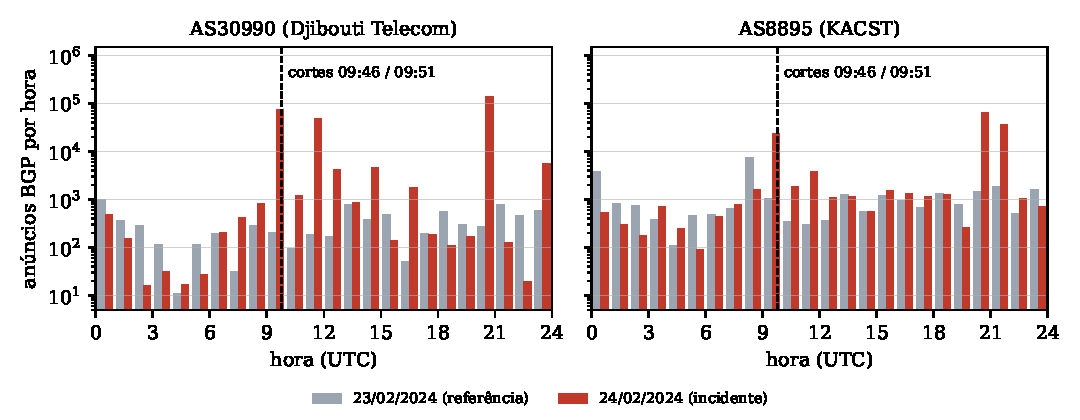
\includegraphics[width=\textwidth]{figuras/update_activity.pdf}
\caption{Anúncios BGP por hora recebidos pelo RIPE RIS para os prefixos de AS30990 e AS8895, em 23/02/2024 (referência) e 24/02/2024, em escala logarítmica. Gráfico do grupo a partir de RIPEstat \textit{BGP Update Activity}, \texttt{resource=AS30990} e \texttt{AS8895}, janela 00:00--24:00~UTC, \texttt{max\_samples=24}. Consulta realizada em 02/11/2026.}
\label{fig:evidencia}
\end{figure}

A evidência reproduzida vem da API do RIPEstat \cite{ripestat2026}, consulta
\url{https://stat.ripe.net/data/bgp-update-activity/data.json?resource=AS30990&starttime=2024-02-24T00:00&endtime=2024-02-25T00:00&max_samples=24},
repetida para AS8895 e para 23/02. Na hora 09:00--09:59~UTC, os anúncios para os prefixos
da Djibouti Telecom saltaram para 73\,336, mais de duas ordens de grandeza acima do mesmo
horário do dia anterior (203); para a KACST, de 1\,029 para 23\,192
(Figura~\ref{fig:evidencia}). Cada coletor que perde o caminho via Tata ou Cogent e aprende
o alternativo gera um anúncio por prefixo. A resolução é de uma hora e não separa os cortes
de 09:46 e 09:51, e há picos às 11:00 (48\,601) e às 20:00 (140\,773 em AS30990; 63\,993 em AS8895) que as fontes não explicam; as consultas minuto a minuto (\textit{BGP Updates} de 197.241.0.0/20 e
102.213.16.0/23) retornaram zero atualizações para a data.

\begin{table}[htb]
\centering
\caption{Vizinhos ``à esquerda'' (\textit{upstreams}) de AS30990 vistos pelo RIS: número de pares que observam o caminho via cada AS. RIPEstat \textit{ASN Neighbours}, \texttt{resource=AS30990}, \texttt{starttime} indicado. Consulta realizada em 02/11/2026.}
\label{tab:vizinhos}
\footnotesize
\begin{tabular}{@{}lrrrrr@{}}
\toprule
\textbf{Upstream} & \textbf{24/02 00:00} & \textbf{24/02 08:00} & \textbf{24/02 16:00} & \textbf{25/02 00:00} & \textbf{02/11/2026} \\
\midrule
AS174 (Cogent)          & 135\,733 & 135\,380 & 72\,789 & 64\,289 & 47\,711 \\
AS6762 (TI Sparkle)     & 13\,550  & 13\,511  & 29\,401 & 72\,521 & 28\,391 \\
AS3356 (Lumen)          & 18\,844  & 18\,768  & 49\,386 & 15\,337 & 16\,387 \\
AS6939 (Hurricane El.)  & 2\,290   & 2\,286   & 1\,170  & 1\,173  & 8\,301 \\
AS23764                 & 245      & 244      & 289     & 281     & 25\,306 \\
\midrule
Vizinhos à esquerda     & 22 & 22 & 10 & 10 & 24 \\
\bottomrule
\end{tabular}
\end{table}

A Tabela~\ref{tab:vizinhos}, feita com as cópias de 8\,h, mostra a migração de AS174
para AS6762 e AS3356, com AS6762 já como caminho mais visto em 25/02. A queda de 22 para 10
vizinhos sugere que a Djibouti Telecom perdeu também sessões com redes europeias menores,
provavelmente alcançadas pelo AAE-1 (inferência). Já os prefixos de AS8895 aparecem em
todas as cópias de 23/02 16:00 a 25/02 16:00: a retirada relatada pela Kentik começou e
terminou entre duas cópias, limitação esperada desse widget.

No \textbf{estado atual} (02/11/2026), os prefixos testados têm ROA válida \cite{rfc6811}:
197.241.0.0/20 e 41.189.224.0/24 (AS30990, ROAs de /17 e /19 com \textit{maxLength} 24),
212.138.84.0/23 (AS8895) e 41.222.60.0/23 (AS37143); 102.213.16.0/23 (AS329242) não tem ROA
(\textit{unknown}). No MANRS \cite{manrs2026}, a rede da KACST (hoje \textit{Saudi Research
\& Innovation Network}) participa desde outubro de 2023 e a Telecom Italia Sparkle desde
julho de 2025; Djibouti Telecom, Etisalat, VNPT, Arusha Art e Simbanet não constam da
lista consultada. Os \textit{upstreams} mudaram: AS30990 tem 24 vizinhos à esquerda e
AS23764 passou de 245 para 25\,306 pares, peso comparável ao da Cogent; AS8895 mantém
Lumen, Tata, GTT e Telecom Italia; AS37143 tem hoje um único vizinho à esquerda (AS36930),
menos redundância que em 2024.

% =====================================================================
\section{Avalia\c{c}\~ao das fontes}
\label{sec:fontes}

O \emph{evento físico} é afirmado pelo operador: a SEACOM confirmou o dano e o segmento
\cite{seacom2024a}, e a HGC, cliente de capacidade, confirmou quatro sistemas danificados
\cite{hgc2024b}; os consórcios do AAE-1 e do EIG não publicaram nada, e não há post-mortem
com instantes. Os \emph{horários} são afirmados por terceiros com evidência (inferidos pela
Kentik do BGP e do IODA); nossos dados horários são compatíveis, mas não os confirmam no
minuto. A \emph{causa} (âncora do \textit{Rubymar}) é hipótese de terceiros, apoiada na
coincidência entre a deriva e os cortes; o Ministério das Telecomunicações controlado pelos
houthis negou envolvimento \cite{madory2024}, e nenhuma fonte primária a confirma. Para
fechar a análise faltariam o relatório dos navios de reparo (posição e marcas de âncora),
que só consórcios e empresa de reparo têm; os dados AIS da trajetória do navio, com as
autoridades marítimas; e os alarmes dos terminais de linha, que dariam o instante exato do
corte e permitiriam medir o atraso até o BGP. As fontes também não dizem quanto da
capacidade de Cogent, Arelion e NTT estava em cada cabo: atribuí-la ao AAE-1 é inferência
pela coincidência de horários. Os comunicados da SEACOM foram lidos em reproduções da imprensa.

% =====================================================================
\section{Li\c{c}\~oes e proje\c{c}\~ao}

Se ocorresse hoje, o efeito no roteamento seria \textbf{semelhante}, e o reparo
provavelmente tão lento quanto. RPKI e filtragem não mudam nada aqui, pois não há anúncio
indevido: o problema é capacidade física. Algumas redes diversificaram (AS30990), mas o
corredor segue concentrado: em setembro de 2025, cortes do SMW4 e do IMEWE no mesmo mar
reduziram em até 28\% o tráfego da Etisalat e em 25\% a 30\% o de regiões do Paquistão,
e elevaram em 20\% a 30\% a latência Índia--Europa \cite{belson2025}.

O Brasil também concentra a capacidade internacional em poucas aterrissagens, e redes
regionais costumam depender de um único traçado de fibra. Propomos duas medidas. \textbf{(1) Diversidade física comprovada de
\textit{upstreams}}: dois trânsitos (ou trânsito e RNP/IX.br) com o traçado físico e os
SRLGs de cada circuito exigidos em contrato \cite{rfc4202} e entradas de fibra por rotas
distintas. Custo: o segundo circuito e a porta no roteador (estimativa do grupo: alguns
milhares de reais por mês para um provedor regional) e a análise do traçado. Limitação:
provedores raramente divulgam o traçado, e dois provedores ``diferentes'' podem alugar
fibra do mesmo \textit{backbone}. \textbf{(2) Anúncio e \textit{failover} sem pontos
únicos}: anunciar todos os prefixos por todos os \textit{upstreams}, fazendo engenharia de
tráfego com \textit{prepending} ou \textit{communities} em vez de anunciar blocos por um só
provedor (o erro da KACST); usar BFD \cite{rfc5880}; seguir a RFC~7454 \cite{rfc7454}; e testar o \textit{failover} em janelas de
manutenção. Custo: baixo, horas de engenharia, desde que cada enlace suporte a carga total.
Limitação: não ajuda se todos os enlaces compartilham o mesmo caminho físico.

% =====================================================================
\section*{Declara\c{c}\~ao de uso de IA generativa}
[[Revisar antes da entrega.]] O grupo usou o Claude (Anthropic) como apoio à pesquisa de
fontes, à execução das consultas à API do RIPEstat, à redação de uma primeira versão do
texto e à geração do gráfico da Figura~\ref{fig:evidencia} e do código do diagrama da
Figura~\ref{fig:mecanismo}. O grupo conferiu as consultas nas próprias ferramentas,
revisou o texto e é responsável pelo conteúdo técnico e pelas conclusões.

% =====================================================================
\IfFileExists{sbc.bst}{\bibliographystyle{sbc}}{\bibliographystyle{plain}}
\bibliography{referencias}

\end{document}
